\documentclass[aspectratio=169, 11pt]{beamer}
\usetheme{default}
\usecolortheme{spruce}
\setbeamertemplate{navigation symbols}{}
\setbeamertemplate{footline}[frame number]

\usepackage{booktabs}
\usepackage{tikz}
\usetikzlibrary{arrows.meta, positioning}

\title[Short Title]{A Beamer Presentation Template}
\subtitle{Academic talks with \LaTeX}
\author{Your Name}
\institute{Example University}
\date{\today}

\begin{document}

\begin{frame}
  \titlepage
\end{frame}

\begin{frame}{Outline}
  \tableofcontents
\end{frame}

\section{Introduction}

\begin{frame}{Why Beamer?}
  \begin{itemize}
    \item Consistent, professional slide decks straight from \LaTeX{}
    \item Math typesetting everywhere: $e^{i\pi} + 1 = 0$
    \item Blocks, columns, and overlays:
  \end{itemize}
  \begin{block}{Key Point}
    Beamer keeps your slides in version control — no binary files.
  \end{block}
\end{frame}

\section{Results}

\begin{frame}{A Figure and a Table}
  \begin{columns}
    \begin{column}{0.48\textwidth}
      \centering
      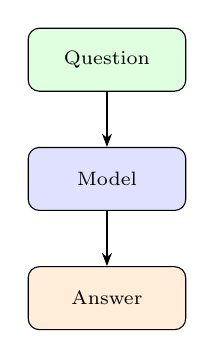
\begin{tikzpicture}[scale=0.8, every node/.style={font=\scriptsize}]
        \node[draw, rounded corners, fill=green!12, minimum width=2cm, minimum height=0.8cm] (q) {Question};
        \node[draw, rounded corners, fill=blue!12, minimum width=2cm, minimum height=0.8cm, below=0.7cm of q] (m) {Model};
        \node[draw, rounded corners, fill=orange!15, minimum width=2cm, minimum height=0.8cm, below=0.7cm of m] (a) {Answer};
        \draw[-{Stealth}] (q) -- (m);
        \draw[-{Stealth}] (m) -- (a);
      \end{tikzpicture}
    \end{column}
    \begin{column}{0.48\textwidth}
      \begin{table}
        \centering
        \begin{tabular}{lcc}
          \toprule
          Method & Acc. & F1 \\
          \midrule
          Base & 81 & 0.79 \\
          Ours & \textbf{88} & \textbf{0.87} \\
          \bottomrule
        \end{tabular}
      \end{table}
    \end{column}
  \end{columns}
\end{frame}

\begin{frame}
  \centering
  {\Huge Thank you!}\\[1em]
  Questions welcome.
\end{frame}

\end{document}
